\section{Appendix: simulation catalog and fact sheets}\label{sec:anexo}

Table~\ref{tab:catalogo} lists the 65 screening, full-city and quadrature simulations; the 19 campus microsimulations are described in the text. Each key simulation then has a fact sheet with its figure: simulated mud (maximum thickness) over the official affected area from IDE Chile and the affected street centerlines, what it tests, what it shows, what limitations it has and what hypotheses it raises. Tests v25 to v29 and the campus microsimulations are summarized in Sections~\ref{sec:res-ronda} and~\ref{sec:res-posterior}; v22 to v24 were stopped before completion (experiment log).

{\scriptsize\setlength{\tabcolsep}{2.5pt}
\begin{longtable}{lll>{\raggedright\arraybackslash}p{3.3cm}rlrrrrrrr}
\caption{Catalogue of the 65 screening, full-city and quadrature simulations (the 19 campus microsimulations are described in Section~\ref{sec:res-posterior}), ordered by exploratory compatibility index (ECI). Culvert capacities and scenarios without fire are calculation assumptions; they do not describe real structures or establish counterfactuals for the event. Columns as in Table~\ref{tab:v4}; runs with the normal time step whose ``sites'' component depends on the campus control point are not used for selection with their raw ECI: without that point they obtain 71--76, unless verified with a fine time step (z26: 76; z29: 78) (protocol amendment 1); v31 was discarded (main channel injection outside the ravine bottom); runs following the held-out test concern fitting; Date: day and month when the simulation ended (2026). Terrain: city (42,018 buildings), previous (1,103 buildings), prev.+ch. (previous terrain with the linear-park channel carved) or SPOT 2014.}\label{tab:catalogo}\\\toprule
Terr. & Date & Run & Scenario & $V$ (thousand m$^3$) & Mud & Streets & Sites & dPH (m) & Perim. & QH & UCC (m) & ECI\\\midrule\endfirsthead
\toprule Terr. & Date & Run & Scenario & $V$ (thousand m$^3$) & Mud & Streets & Sites & dPH (m) & Perim. & QH & UCC (m) & ECI\\\midrule\endhead
city & 11-10 & v26 & channel + southern branches; porous houses in the official area + net rainfall & 300 & G2b & 0.77 & 1.00 & 1 & 0.54 & 0.56 & 0.30 & 83\\
city & 12-10 & v30 & channel + southern branches; porous houses, Kp 1000 and n 0.1 (v26 sensitivity) & 300 & G2b & 0.76 & 1.00 & 1 & 0.53 & 0.54 & 0.31 & 82\\
city & 12-10 & v32 & channel + southern branches; integrated hypothesis: porous houses, turbid water on the lower hillside, road, La Plaza Sur and university entrances & 300 & G2b & 0.77 & 1.00 & 1 & 0.51 & 0.56 & 0.30 & 82\\
city & 12-10 & z32 & channel + southern branches; integrated hypothesis, fine time step & 300 & G2b & 0.77 & 1.00 & 5 & 0.51 & 0.56 & 0.30 & 82\\
city & 13-10 & f35 & channel + southern branches; as p34, without fire: 187 thousand m$^3$ and Qp 172 m$^3$/s; with a +3.1 \% artifact, repeated as f35b/f38b & 187 & G2b & 0.73 & 1.00 & 5 & 0.53 & 0.56 & 0.23 & 82\\
city & 13-10 & m36 & channel + southern branches; as p34, with a fine mesh (8 m$^2$) on the campus and La Plaza Sur & 300 & G2b & 0.78 & 1.00 & 6 & 0.48 & 0.52 & 0.32 & 82\\
city & 13-10 & f35b & channel + southern branches; corrected repeat of f35, without fire & 187 & G2b & 0.73 & 1.00 & 5 & 0.55 & 0.56 & 0.23 & 82\\
city & 13-10 & d39 & channel + southern branches; as p34, only houses of 250 m$^2$ or less are porous & 300 & G2b & 0.77 & 1.00 & 5 & 0.47 & 0.55 & 0.31 & 81\\
city & 13-10 & p34 & channel + southern branches; integrated hypothesis with Río Molina rainfall measured every 30 min (31.8 mm); with a +2.1 \% mass artifact, repeated without it as p34b & 300 & G2b & 0.77 & 1.00 & 1 & 0.48 & 0.56 & 0.30 & 81\\
city & 13-10 & p34b & channel + southern branches; corrected repeat of p34 (maximum time step 0.5 s, residual 0.00 \%) & 300 & G2b & 0.77 & 1.00 & 1 & 0.48 & 0.56 & 0.30 & 81\\
city & 13-10 & f38 & channel + southern branches; as f35, more fluid mud (Cv 0.25); with a +3.1 \% artifact, repeated as f35b/f38b & 187 & G2b & 0.70 & 1.00 & 5 & 0.49 & 0.54 & 0.19 & 80\\
city & 13-10 & f38b & channel + southern branches; corrected repeat of f38, without fire and with more fluid mud & 187 & G2b & 0.70 & 1.00 & 5 & 0.50 & 0.54 & 0.19 & 80\\
city & 11-10 & v27 & channel + southern branches; greater roughness in gardens and trees + rainfall & 300 & G2b & 0.78 & 1.00 & 8 & 0.39 & 0.68 & 1.13 & 79\\
city & 12-10 & v33 & channel + southern branches; integrated hypothesis with measured rainfall: 8 mm/h for 4 h & 300 & G2b & 0.76 & 1.00 & 1 & 0.41 & 0.56 & 0.30 & 79\\
city & 13-10 & arc & channel + southern branches; as p34, main channel carved along the line of trees and flow injected upstream (hypothetical obstacle control) & 300 & G2b & 0.75 & 1.00 & 5 & 0.40 & 0.56 & 0.24 & 79\\
city & 11-10 & v20 & channel + southern branches; rainfall 35 mm/h + official southern branch (terrain v6), normal time step & 300 & G2b & 0.77 & 1.00 & 15 & 0.33 & 0.68 & 1.12 & 78\\
city & 11-10 & v25 & channel + southern branches; slightly denser mud (Cv 0.43) + rainfall & 300 & G2b & 0.77 & 1.00 & 15 & 0.35 & 0.68 & 1.11 & 78\\
city & 11-10 & v29 & channel + southern branches; liquid flow on lower hillside (Cv 0.27) + main branch Cv 0.43 + net rainfall & 300 & G2b & 0.77 & 1.00 & 15 & 0.35 & 0.68 & 1.11 & 78\\
city & 11-10 & v28 & channel + southern branches; rainfall 35 mm/h only outside contributing catchments (no double counting) & 300 & G2b & 0.77 & 1.00 & 15 & 0.34 & 0.68 & 1.13 & 78\\
city & 11-10 & q3 & channel + southern branches; Cv quadrature: node Cv 0.365 & 300 & G2b & 0.77 & 1.00 & 15 & 0.34 & 0.68 & 1.13 & 78\\
city & 11-10 & q4 & channel + southern branches; Cv quadrature: node Cv 0.429 & 300 & G2b & 0.77 & 1.00 & 15 & 0.36 & 0.68 & 1.12 & 78\\
city & 12-10 & z29 & channel + southern branches; lower hillside Cv 0.27, fine time step & 300 & G2b & 0.77 & 1.00 & 15 & 0.35 & 0.68 & 1.11 & 78\\
city & 12-10 & v31 & channel + southern branches; integrated hypothesis: porous houses, road, La Plaza Sur, university entrances, trees, H1 upstream, lower hillside Cv 0.10 & 300 & G2b & 0.72 & 1.00 & 191 & 0.40 & 0.51 & 0.19 & 78\\
city & 13-10 & art & channel + southern branches; as arc, with a hypothetical log obstacle with an assumed height of 3 m at the end of the line of trees & 300 & G2b & 0.73 & 1.00 & 5 & 0.39 & 0.54 & 0.22 & 78\\
city & 11-10 & q2 & channel + southern branches; Cv quadrature: node Cv 0.297 & 300 & G2b & 0.77 & 1.00 & 15 & 0.32 & 0.68 & 1.14 & 77\\
city & 11-10 & q1 & channel + southern branches; Cv quadrature: node Cv 0.239 & 300 & G2b & 0.76 & 1.00 & 15 & 0.32 & 0.68 & 1.14 & 77\\
city & 12-10 & z26 & channel + southern branches; porous houses, fine time step & 300 & G2b & 0.76 & 0.75 & 5 & 0.54 & 0.56 & 0.30 & 76\\
city & 11-10 & q5 & channel + southern branches; Cv quadrature: node Cv 0.478 & 300 & G2b & 0.78 & 0.75 & 34 & 0.38 & 0.68 & 1.11 & 73\\
city & 10-10 & v02 & channel + southern branches; rainfall 35 mm/h on hillside & 300 & G2b & 0.77 & 0.75 & 15 & 0.34 & 0.68 & 1.13 & 72\\
city & 10-10 & z02 & channel + southern branches; rainfall 35 mm/h, time step 4× finer & 300 & G2b & 0.77 & 0.75 & 15 & 0.34 & 0.68 & 1.13 & 72\\
previous & 09-10 & f03 & arainfalll fan + culvert inlet + southern branches; rainfall 35 mm/h on hillside & 150 & G2b & 0.73 & 0.75 & 225 & 0.39 & 0.66 & 0.26 & 71\\
city & 10-10 & v14 & channel + southern branches; rainfall 35 mm/h + Álvaro del Portillo ravine & 300 & G2b & 0.77 & 0.75 & 15 & 0.34 & 0.68 & 1.15 & 71\\
city & 11-10 & v19 & channel + southern branches; rainfall 35 mm/h + official southern branch to Álvaro del Portillo (terrain v6) & 300 & G2b & 0.77 & 0.75 & 15 & 0.34 & 0.68 & 1.11 & 71\\
city & 10-10 & v09 & main channel & 300 & A2 & 0.77 & 0.50 & 151 & 0.52 & 0.68 & 1.14 & 70\\
city & 10-10 & v03 & main channel; culvert with assumed capacity of 30 m$^3$/s & 300 & G2b & 0.77 & 0.50 & 96 & 0.50 & 0.64 & 1.16 & 69\\
city & 10-10 & v05 & main channel; culvert with assumed capacity of 100 m$^3$/s & 300 & G2b & 0.74 & 0.50 & 96 & 0.53 & 0.44 & 1.16 & 69\\
city & 10-10 & v06 & main channel; culvert with assumed capacity of 60 m$^3$/s & 300 & G2b & 0.74 & 0.50 & 96 & 0.53 & 0.44 & 1.16 & 69\\
city & 10-10 & v17 & main channel; culvert with assumed capacity of 30 m$^3$/s, capture 25 m, Quebrada Honda carved & 300 & G2b & 0.76 & 0.50 & 96 & 0.50 & 0.62 & 1.18 & 69\\
prev.+ch. & 09-10 & f01 & main channel & 150 & G2b & 0.71 & 0.50 & 338 & 0.63 & 0.55 & 0.31 & 68\\
prev.+ch. & 09-10 & e04 & main channel & 300 & G2b & 0.75 & 0.50 & 2 & 0.46 & 0.56 & 0.32 & 68\\
city & 10-10 & v01 & main channel & 300 & G2b & 0.77 & 0.50 & 96 & 0.46 & 0.68 & 1.16 & 68\\
city & 10-10 & z01 & main channel; numerical check (time step 4× finer) & 300 & G2b & 0.77 & 0.50 & 96 & 0.46 & 0.68 & 1.16 & 68\\
city & 10-10 & v10 & main channel; culvert with assumed capacity of 100 m$^3$/s, capture 25 m & 300 & G2b & 0.69 & 0.50 & 96 & 0.52 & 0.00 & 1.16 & 68\\
city & 10-10 & v11 & main channel; culvert with assumed capacity of 200 m$^3$/s, capture 40 m & 300 & G2b & 0.69 & 0.50 & 96 & 0.52 & 0.00 & 1.16 & 68\\
city & 10-10 & v15 & main channel; Quebrada Honda carved downstream (terrain v5) & 300 & G2b & 0.77 & 0.50 & 96 & 0.45 & 0.68 & 1.18 & 68\\
city & 10-10 & v18 & main channel; culvert with assumed capacity of 100 m$^3$/s, capture 25 m, Quebrada Honda carved & 300 & G2b & 0.69 & 0.50 & 96 & 0.52 & 0.00 & 1.18 & 68\\
city & 11-10 & v21 & channel + southern branches; official southern branch (terrain v6), without rainfall & 300 & G2b & 0.77 & 0.50 & 131 & 0.45 & 0.68 & 1.11 & 68\\
prev.+ch. & 09-10 & k03 & main channel; culvert with assumed capacity of 10 m$^3$/s & 150 & G2b & 0.70 & 0.50 & 338 & 0.64 & 0.43 & 0.31 & 67\\
city & 10-10 & v07 & main channel & 150 & G2b & 0.72 & 0.50 & 348 & 0.62 & 0.68 & 1.09 & 67\\
city & 10-10 & v08 & main channel & 300 & G1 & 0.74 & 0.50 & 396 & 0.63 & 0.69 & 1.16 & 67\\
prev.+ch. & 09-10 & k01 & main channel; culvert with assumed capacity of 30 m$^3$/s & 150 & G2b & 0.65 & 0.50 & 338 & 0.63 & 0.01 & 0.31 & 66\\
prev.+ch. & 09-10 & k02 & main channel; culvert with assumed capacity of 100 m$^3$/s & 150 & G2b & 0.65 & 0.50 & 338 & 0.63 & 0.01 & 0.31 & 66\\
previous & 09-10 & d02 & channel + southern branches & 300 & G2b & 0.68 & 0.50 & 4 & 0.41 & 0.00 & 0.42 & 65\\
previous & 09-10 & d04 & main channel & 150 & G2b & 0.63 & 0.50 & 366 & 0.55 & 0.00 & 0.42 & 63\\
previous & 09-10 & d01 & channel + southern branches & 150 & G2b & 0.60 & 0.50 & 516 & 0.55 & 0.00 & 0.39 & 58\\
previous & 09-10 & g01 & channel + southern branches & 150 & G2b & 0.58 & 0.50 & 592 & 0.51 & 0.00 & 0.38 & 55\\
previous & 09-10 & g03 & arainfalll fan + culvert inlet + southern branches & 150 & G2b & 0.60 & 0.50 & 816 & 0.53 & 0.54 & 0.35 & 50\\
previous & 09-10 & f02 & arainfalll fan + culvert inlet + southern branches; rainfall 20 mm/h on hillside & 150 & G2b & 0.56 & 0.75 & 1,005 & 0.46 & 0.66 & 0.26 & 49\\
previous & 09-10 & g02 & arainfalll fan + culvert inlet + southern branches & 150 & G2b & 0.61 & 0.50 & 947 & 0.51 & 0.57 & 0.33 & 47\\
previous & 09-10 & e06 & main channel & 150 & G1 & 0.47 & 0.50 & 1,686 & 0.80 & 0.45 & 0.59 & 44\\
previous & 09-10 & d03 & channel + southern branches; peak discharge 100 m$^3$/s & 80 & G2b & 0.50 & 0.50 & 1,160 & 0.68 & 0.00 & 0.22 & 43\\
previous & 09-10 & e01 & arainfalll fan + culvert inlet + southern branches & 150 & G2b & 0.56 & 0.50 & 1,007 & 0.46 & 0.66 & 0.26 & 43\\
previous & 09-10 & e02 & arainfalll fan + culvert inlet + southern branches & 150 & G2b & 0.52 & 0.50 & 982 & 0.43 & 0.67 & 0.23 & 42\\
SPOT 2014 & 09-10 & s01 & main channel & 150 & G2b & 0.50 & 0.50 & 1,188 & 0.60 & 0.77 & 0.37 & 40\\
previous & 09-10 & e03 & culvert inlet only & 150 & G2b & 0.08 & 0.00 & 856 & 0.20 & 0.69 & 0.00 & 16\\
\bottomrule\end{longtable}}


\subsection*{Tests following the held-out test (fitting)}

\paragraph{v32 · Integrated hypothesis: porous houses, turbid water on the lower hillside and campus features.} \textbf{What it tests:} It combines what was learned after the held-out test: houses in the official area that allow mud to enter, turbid water (Cv 0.10) on the lower hillside of the campus and La Plaza Sur, mud with Cv 0.40 in the main branch, and features unresolved by the 30 m terrain (hillside road, lower roadway of La Plaza Sur, university and parking lot entrances), with rainfall over the entire lower hillside outside the contributing catchments. \textbf{What it shows:} Calculated: it meets the four original acceptance criteria (ECI 82/100; the repeat run with a fine time step, z32, gives the same value); urban mud within the official area reaches 51 \%; the campus records 0.61 m; La Plaza Sur is wetted along 46 \% of its length; in the model, water enters through the clearing into the courtyard (0.07 m) and the parking lot. \textbf{Model limitations:} Next to the UC Christus emergency department it calculates 0.30 m (Cadena 3 reported about 1 m in the emergency department). On campus, with the city mesh, less water arrives than in the detailed simulations; with a fine mesh on campus (m36), the courtyard reaches 0.17 m, attributing the difference to resolution. It is conditional on rainfall of 35 mm/h for one hour, greater than the measured rainfall: with the measured rainfall it scores 79/100 (distributed evenly) or 81/100 (with its pulse shape). \textbf{What it raises:} In the model, different properties are assigned to flow in the main branch and on campus; assumed retention within lots modifies the calculated distribution within the official area. The fit does not identify the processes that occurred during the event. \textbf{Status:} ECI 82/100 verified with a fine time step (z32). Fitting after the held-out test.

\begin{figure}[H]\centering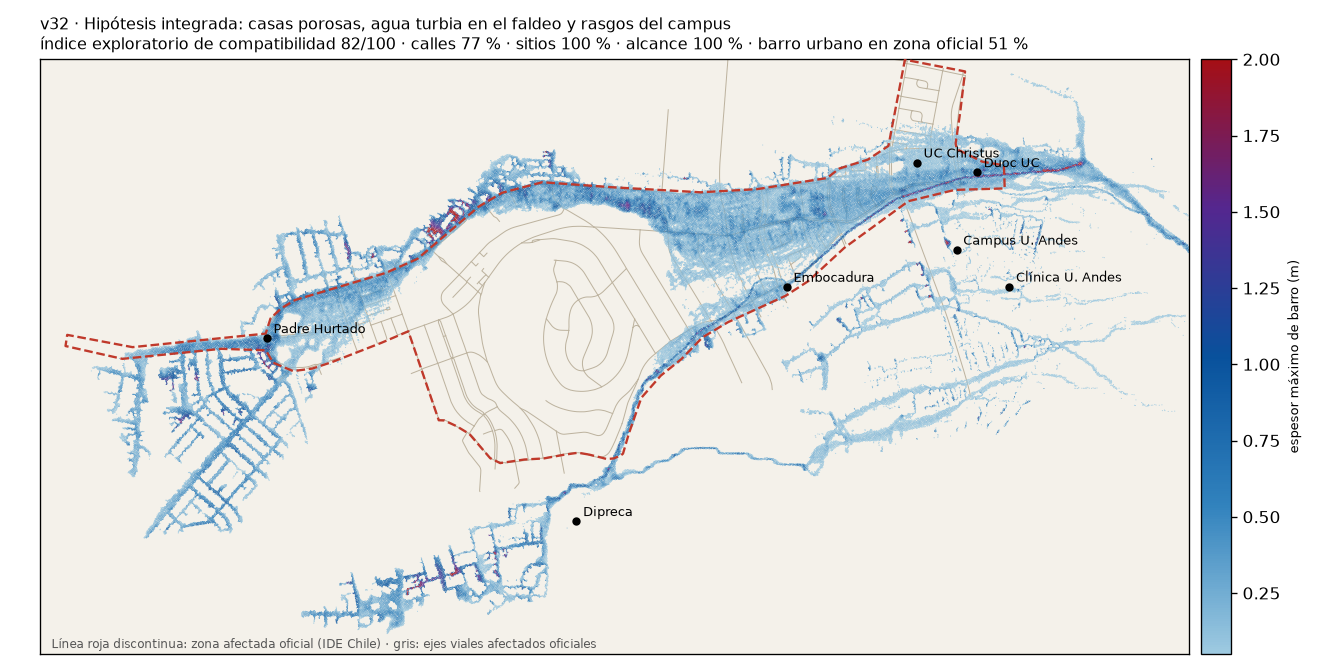
\includegraphics[width=\textwidth]{anexo/v32}\caption{Fact sheet v32: Integrated hypothesis: porous houses, turbid water on the lower hillside and campus features.}\end{figure}

\paragraph{z26 · Porous houses (fine time step).} \textbf{What it tests:} Allowing buildings in the official area to admit mud (floor at ground elevation plus 0.3 m and high resistance), instead of representing them as solid blocks. \textbf{What it shows:} Calculated: urban mud within the official area increases from 34 \% to 54 \%; it wets 36 \% of the official area and 40 \% of its affected properties; it meets the four original acceptance criteria. With half the resistance (v30), there is almost no change. \textbf{Model limitations:} The calculated depth next to the UC Christus emergency department drops to 0.30 m. The campus point remains dry with a fine time step. \textbf{What it raises:} In the model, assumed mud retention within lots modifies the calculated distribution within the official area; its representation remains an assumption. \textbf{Status:} ECI verified with a fine time step: 76/100 (subsequent fitting).

\begin{figure}[H]\centering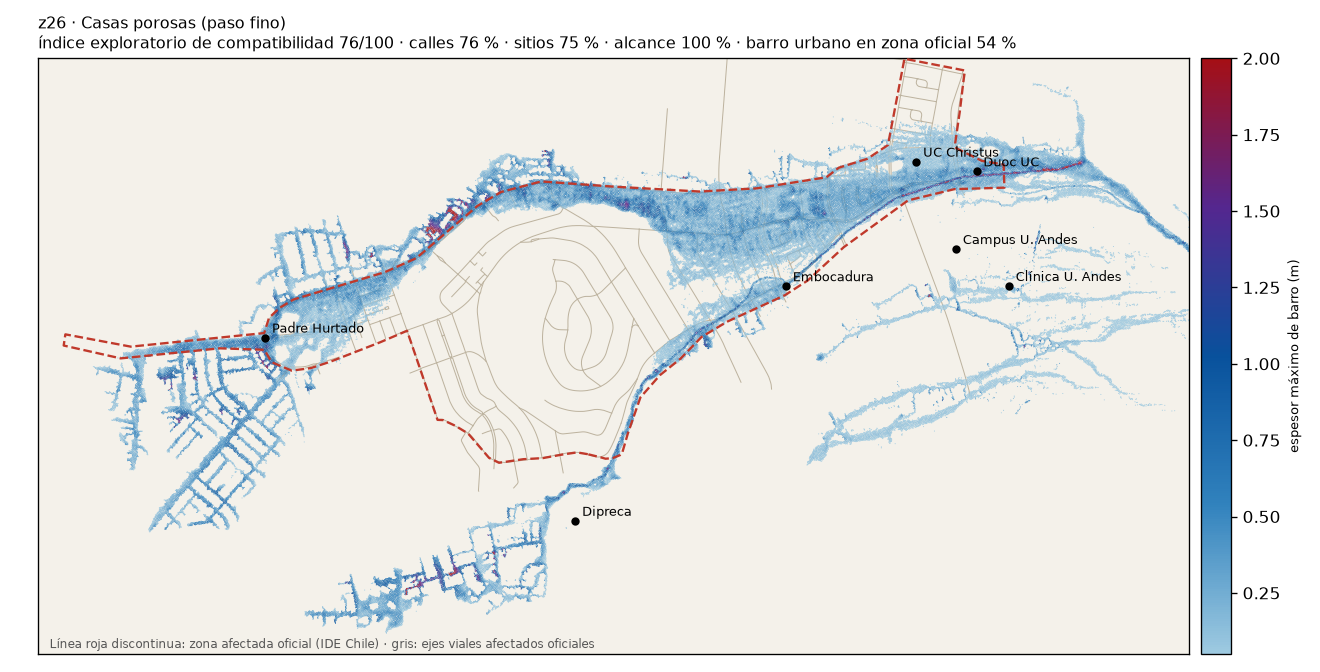
\includegraphics[width=\textwidth]{anexo/z26}\caption{Fact sheet z26: Porous houses (fine time step).}\end{figure}

\paragraph{z29 · More liquid fluid on the lower hillside (fine time step).} \textbf{What it tests:} Two mud mixtures depending on the area: Cv 0.27 on the lower hillside of the campus and Cv 0.43 in the main branch, with rainfall only outside the contributing catchments. \textbf{What it shows:} Calculated: the campus control point remains wet with a fine time step (0.09 m), unlike the hypothesis with a single mud mixture (0.01 m). \textbf{Model limitations:} It does not reduce mud outside the official area: the fraction within it remains at 0.35. \textbf{What it raises:} In these tests, an assumed more liquid fluid on the lower hillside, compatible with the turbid water interpreted in the Meganoticias video, also produces flow on campus with a fine time step. \textbf{Status:} ECI verified with a fine time step: 78/100 (subsequent fitting).

\begin{figure}[H]\centering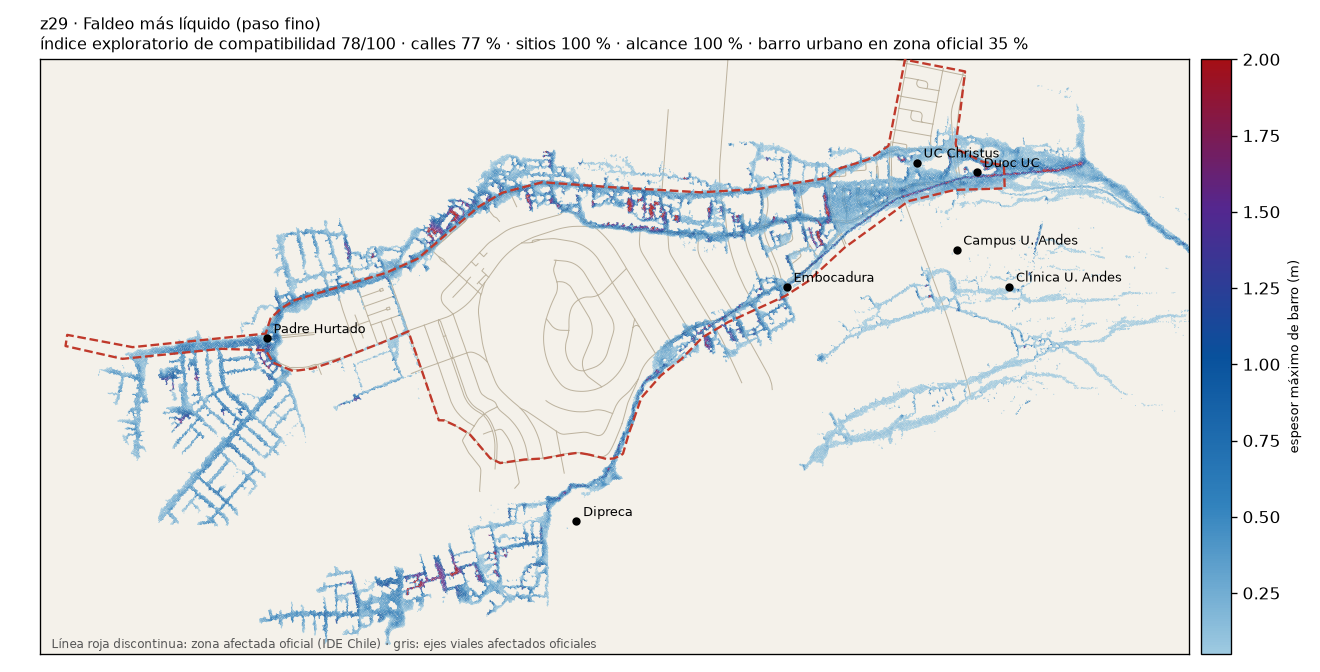
\includegraphics[width=\textwidth]{anexo/z29}\caption{Fact sheet z29: More liquid fluid on the lower hillside (fine time step).}\end{figure}

\subsection*{Hypothesis selected for the held-out test}

\paragraph{z02 · Channel + southern branches + hillside rainfall, full city (fine time step).} \textbf{What it tests:} The hypothesis selected before the test with held-out observations: mud emerges through the main channel onto the alluvial fan and through the southern branches, with rainfall of 35 mm/h also applied over the burned hillside. It repeats v02 with a time step four times finer to examine sensitivity to the time step. \textbf{What it shows:} Calculated: simulated flow follows the two corridors delimiting the official area (El Alba–General Blanche and Quebrada Honda) and comes within 200 m of Padre Hurtado; around Clínica UC Christus it calculates 1.13 m (Cadena 3 reported about 1 m in the emergency department) and produces flow next to Clínica U. de los Andes. The indicators match those of v02; this numerical check does not validate the event reconstruction. \textbf{Model limitations:} Only one third of simulated mud in urban areas falls within the official area: it extends west of Padre Hurtado, along Quebrada Honda towards Dipreca and, because of the applied rainfall, along streets in other neighborhoods. It does not reach the U. de los Andes campus. Part of the applied rainfall (about 9,400 m$^3$) overlaps catchments already entering through the hydrographs; v28 corrects this. \textbf{What it raises:} In z02, hillside rainfall contributes to reproducing flow next to the clinic; the result does not establish its contribution during the event. Building representation, coarse load and vegetation are considered possible explanations for the extent outside the official area (v25–v27). \textbf{Status:} Hypothesis selected before the test with held-out observations (unfavorable test result): ECI 72/100. Subsequent tests (porous houses, liquid fluid on the lower hillside, integrated hypothesis) outperform it through fitting.

\begin{figure}[H]\centering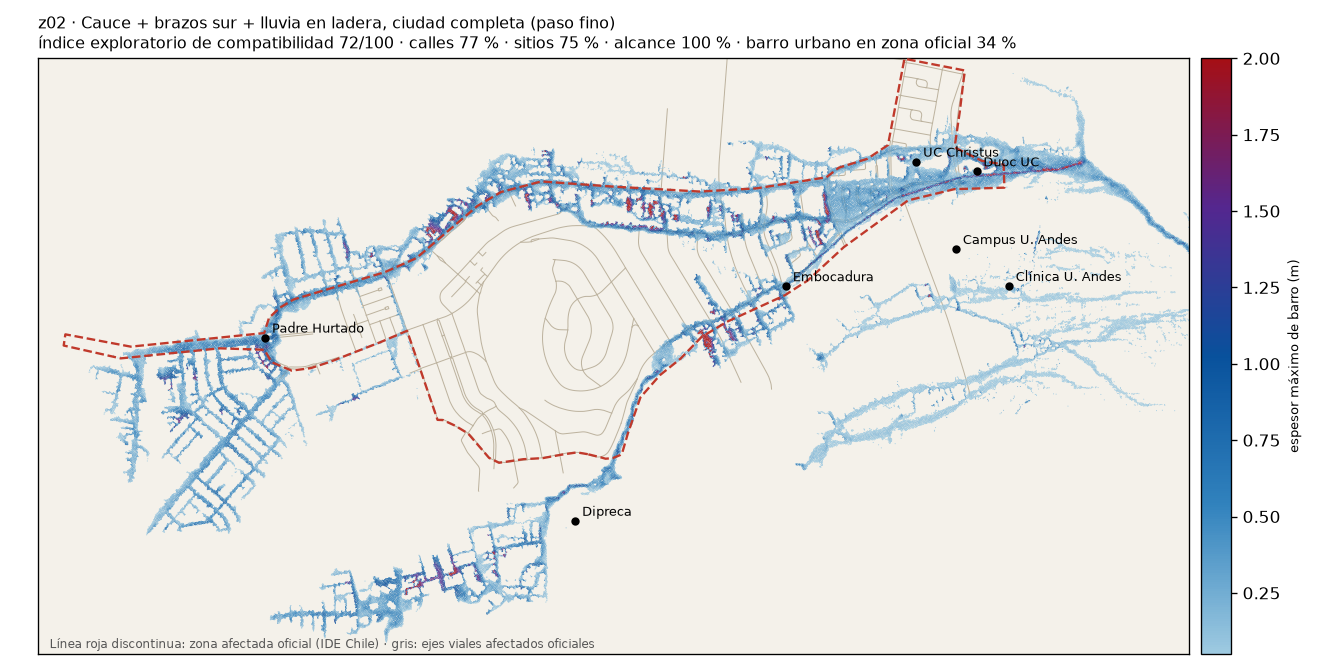
\includegraphics[width=\textwidth]{anexo/z02}\caption{Fact sheet z02: Channel + southern branches + hillside rainfall, full city (fine time step).}\end{figure}

\subsection*{Full city}

\paragraph{v01 · Main channel only, culvert with assumed zero capacity (300 thousand m$^3$).} \textbf{What it tests:} All mud emerges through the main channel onto the alluvial fan, with the General Blanche conduits and the Bulnes Correa culvert assumed to have zero capacity (hypothetical scenario). \textbf{What it shows:} Calculated: with the 42 thousand buildings, flow is channeled along streets; it calculates 1.16 m around UC Christus (0.3 m with the previous terrain), 1.9 m next to Duoc UC, comes within 96 m of Padre Hurtado and wets Quebrada Honda. \textbf{Model limitations:} It does not reproduce impacts next to Clínica U. de los Andes, on La Plaza Sur or on the campus. \textbf{What it raises:} This configuration does not reproduce impacts in the southern sector. Inflows from that sector are one of the hypotheses considered to explain the discrepancy. \textbf{Status:} Reference: ECI 68/100.

\begin{figure}[H]\centering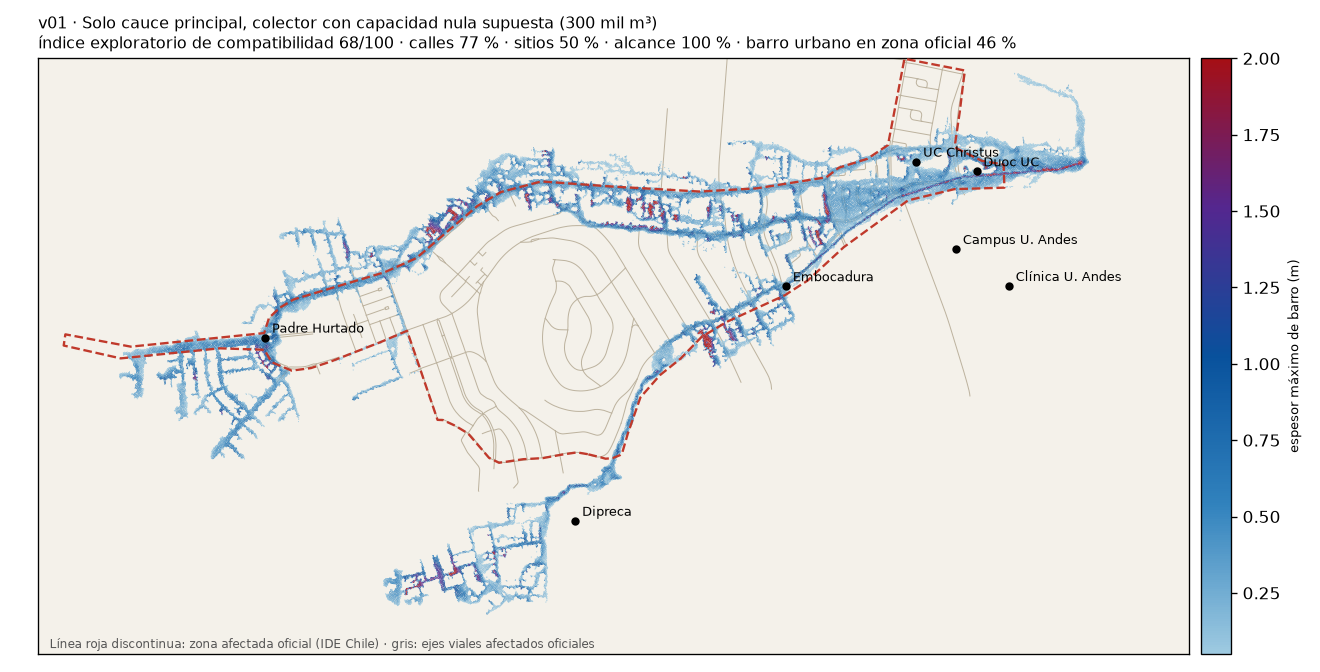
\includegraphics[width=\textwidth]{anexo/v01}\caption{Fact sheet v01: Main channel only, culvert with assumed zero capacity (300 thousand m$^3$).}\end{figure}

\paragraph{v07 · Main channel only with 150 thousand m$^3$.} \textbf{What it tests:} Same as v01, but with half the volume: the central value of the first rainfall-based estimate. \textbf{What it shows:} Calculated: the front stops 348 m from Padre Hurtado. \textbf{Model limitations:} It does not meet the reach criterion. \textbf{What it raises:} In the scenarios tested and under their assumptions, about 300 thousand m$^3$ allows the reach criterion to be reproduced; that order of magnitude is consistent with a rainfall-based estimate adopting the soil saturation reported by the authority. \textbf{Status:} The low-volume configuration does not meet the reach criterion: ECI 67/100.

\begin{figure}[H]\centering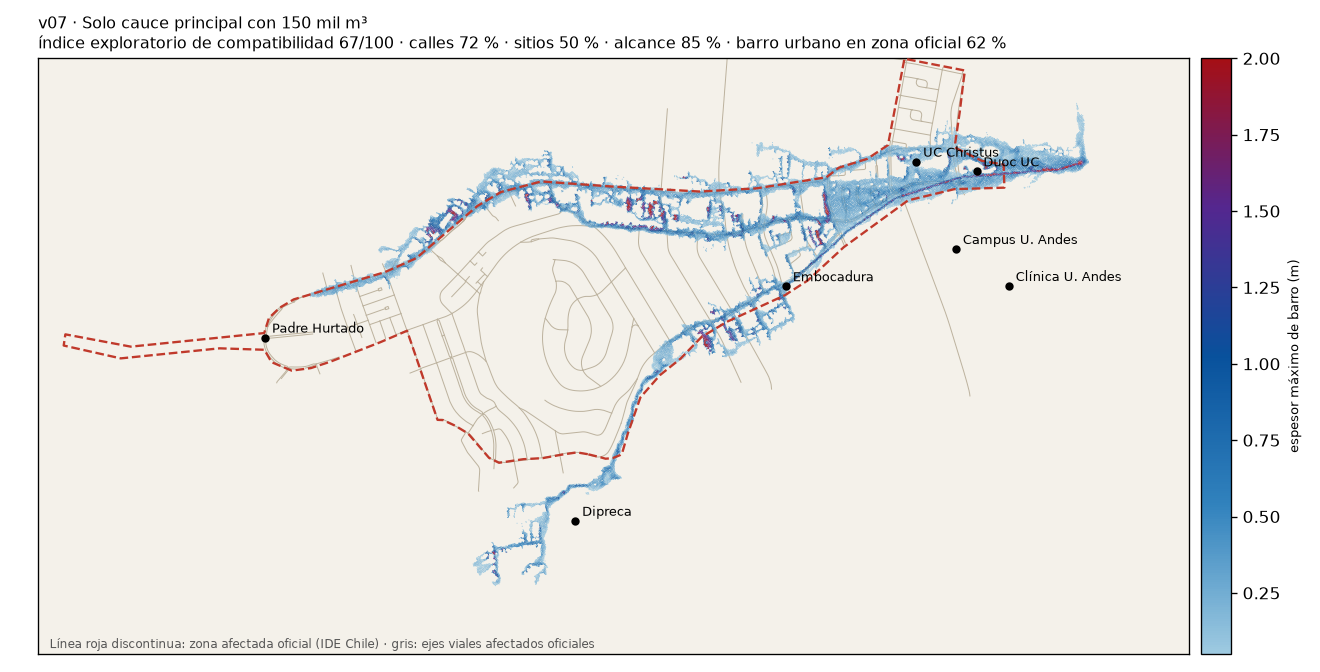
\includegraphics[width=\textwidth]{anexo/v07}\caption{Fact sheet v07: Main channel only with 150 thousand m$^3$.}\end{figure}

\subsection*{U. Andes campus}

\paragraph{v21 · Southern branch along the official channel, without hillside rainfall.} \textbf{What it tests:} The southern branch follows the official hydrographic network alignment to upper Av. Álvaro del Portillo, where the official alignment ends and the model allows flow to discharge onto the avenue. Without hillside rainfall, to isolate its effect. \textbf{What it shows:} Calculated: mud from the southern branch reaches the avenue (0.48 m where the channel ends) and runs down it towards La Plaza and General Blanche, in a manner compatible with what Cooperativa attributed to the vice-rector and La Tercera to Carabineros. \textbf{Model limitations:} Without hillside rainfall, the impact next to Clínica U. de los Andes is not reproduced (0 m) and flow does not reach the Biblioteca. \textbf{What it raises:} In the configurations compared, hillside rainfall allows impacts next to the clinic to be reproduced, and, in the model, the southern branch generates an overflow compatible with the one the vice-rector described to Cooperativa on the north side of the campus. \textbf{Status:} ECI 68/100.

\begin{figure}[H]\centering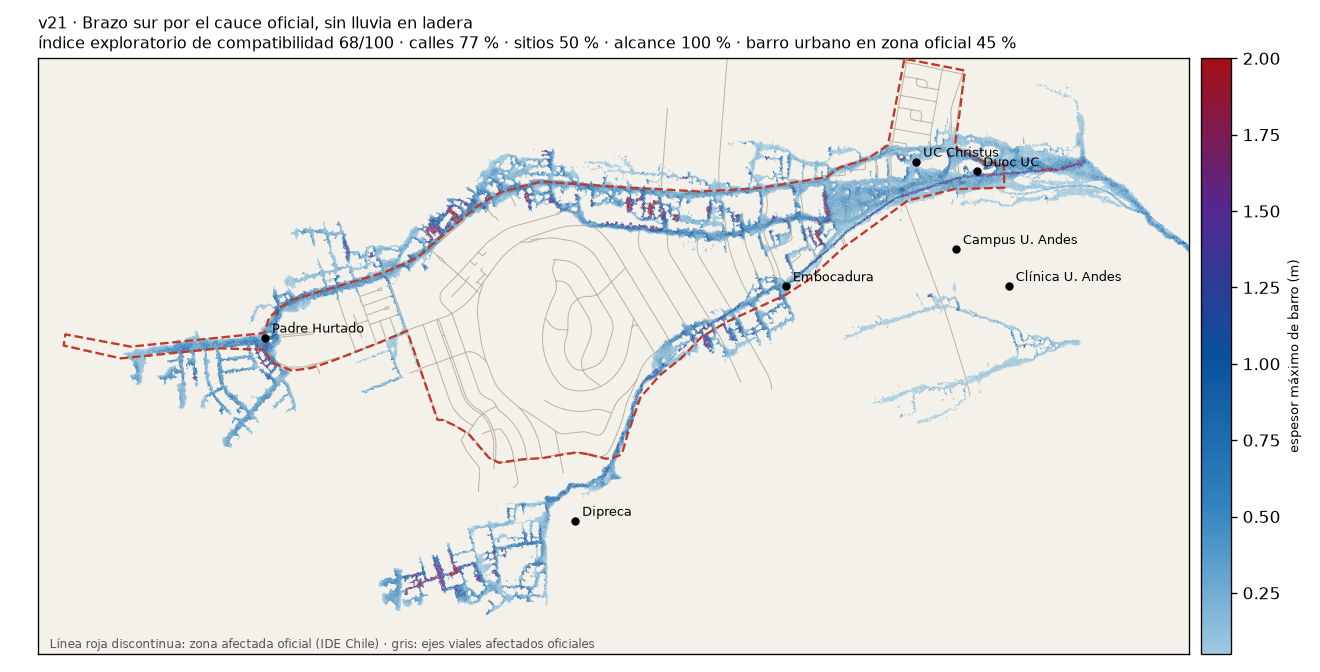
\includegraphics[width=\textwidth]{anexo/v21}\caption{Fact sheet v21: Southern branch along the official channel, without hillside rainfall.}\end{figure}

\paragraph{v19 · Southern branch along the official channel to Álvaro del Portillo + rainfall (fine time step).} \textbf{What it tests:} The selected hypothesis (z02) with the southern branch traced according to official mapping, to examine whether flow reaches the campus and the Aula Magna. \textbf{What it shows:} Calculated: it reproduces an overflow in upper Álvaro del Portillo and its descent along the avenue, in addition to what z02 achieves. \textbf{Model limitations:} Simulated flow continues along the avenue, which is steeper ($\sim$8 \%) than the woodland towards the Biblioteca ($\sim$4 \%), and does not reach the depression next to the building or the campus control point (1 cm). \textbf{What it raises:} In subsequent microsimulations, the assumed overflow does not reach the courtyard with any of the fluids tested; the most compatible scenario assumes turbid hillside runoff that, in the model, follows La Plaza Sur and enters through a clearing, with carved features unresolved by the 30 m terrain. \textbf{Status:} ECI 71/100. Superseded as a fit by the scenario with assumed local runoff input (see v32); the actual origin of the water is not determined.

\begin{figure}[H]\centering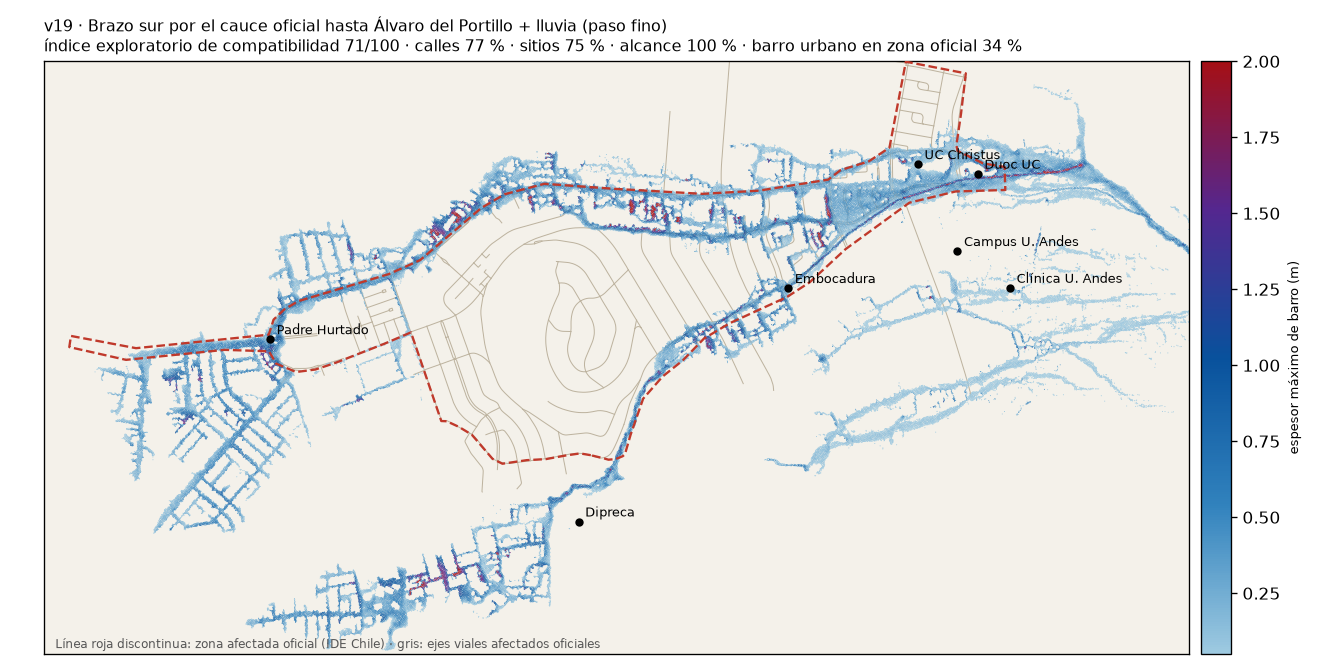
\includegraphics[width=\textwidth]{anexo/v19}\caption{Fact sheet v19: Southern branch along the official channel to Álvaro del Portillo + rainfall (fine time step).}\end{figure}

\subsection*{Bulnes Correa culvert (hypothetical scenarios)}

\paragraph{v17 · Hypothetical scenario: assumed culvert capacity set to 30 m$^3$/s.} \textbf{What it tests:} Hypothetical scenario with assumed culvert capacity set to 30 m$^3$/s and capture of the entire channel cross section. Public information on the actual capacity and condition of the culvert was unavailable. \textbf{What it shows:} Calculated: the modeled culvert reaches the imposed capacity (removes 67.6 thousand m$^3$ at 30 m$^3$/s) and Quebrada Honda is wetted at 62 \% of its points. \textbf{Model limitations:} — \textbf{What it raises:} In the model, with an assumed capacity of 30 m$^3$/s, surface flow remains towards Quebrada Honda. This is not an evaluation of the real structure. \textbf{Status:} Lower reference for the interval explored in these scenarios: ECI 69/100.

\begin{figure}[H]\centering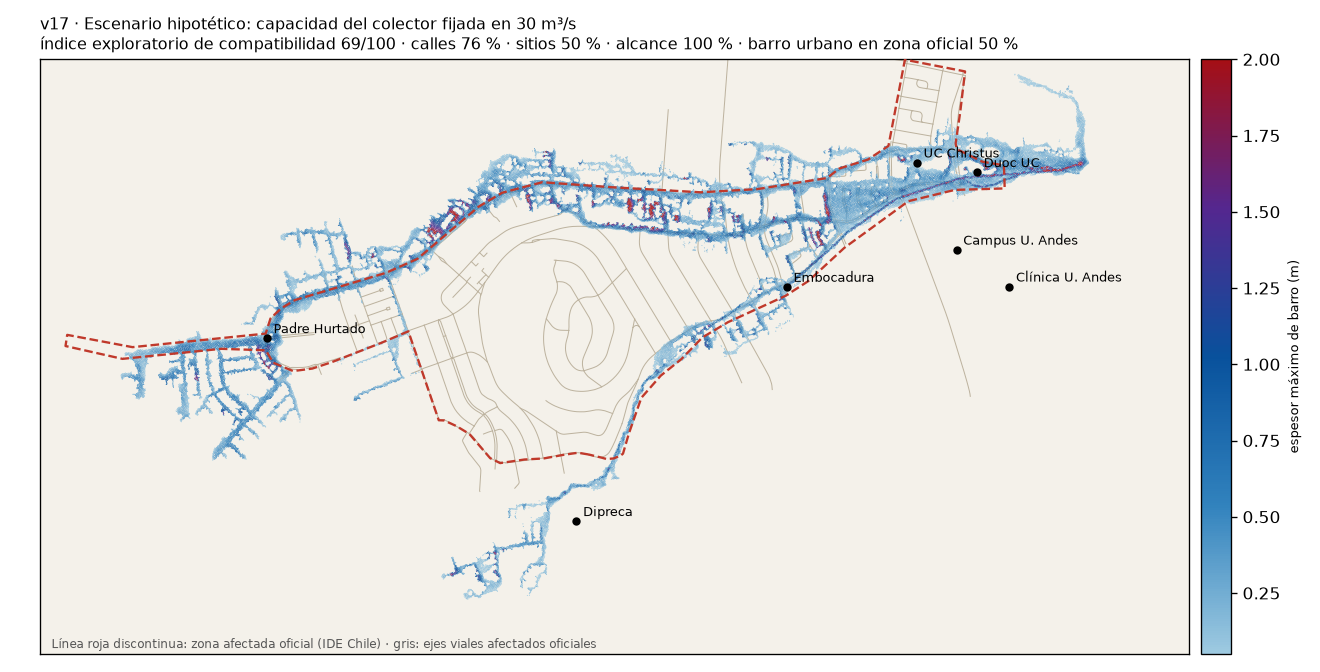
\includegraphics[width=\textwidth]{anexo/v17}\caption{Fact sheet v17: Hypothetical scenario: assumed culvert capacity set to 30 m$^3$/s.}\end{figure}

\paragraph{v10 · Hypothetical scenario: assumed culvert capacity set to 100 m$^3$/s.} \textbf{What it tests:} Hypothetical high-capacity scenario with capture of the entire channel cross section. \textbf{What it shows:} Calculated: the modeled culvert removes about 93 thousand m$^3$ with a peak of $\sim$64 m$^3$/s and Quebrada Honda remains dry. With 200 m$^3$/s the result is the same, because calculated arriving discharge does not exceed $\sim$65 m$^3$/s. \textbf{Model limitations:} The scenario does not reproduce the reported flooding of Quebrada Honda; this discrepancy does not allow the operation of the real culvert to be established. \textbf{What it raises:} Under the assumptions tested and with full capture, the analysis places the calculated threshold of assumed capacity for removing all surface flow in the model near 65 m$^3$/s. A capture radius of 12 m allowed flow to pass beside the sink: this was a representation artifact, now corrected. \textbf{Status:} Upper reference for the interval explored in these scenarios: ECI 68/100.

\begin{figure}[H]\centering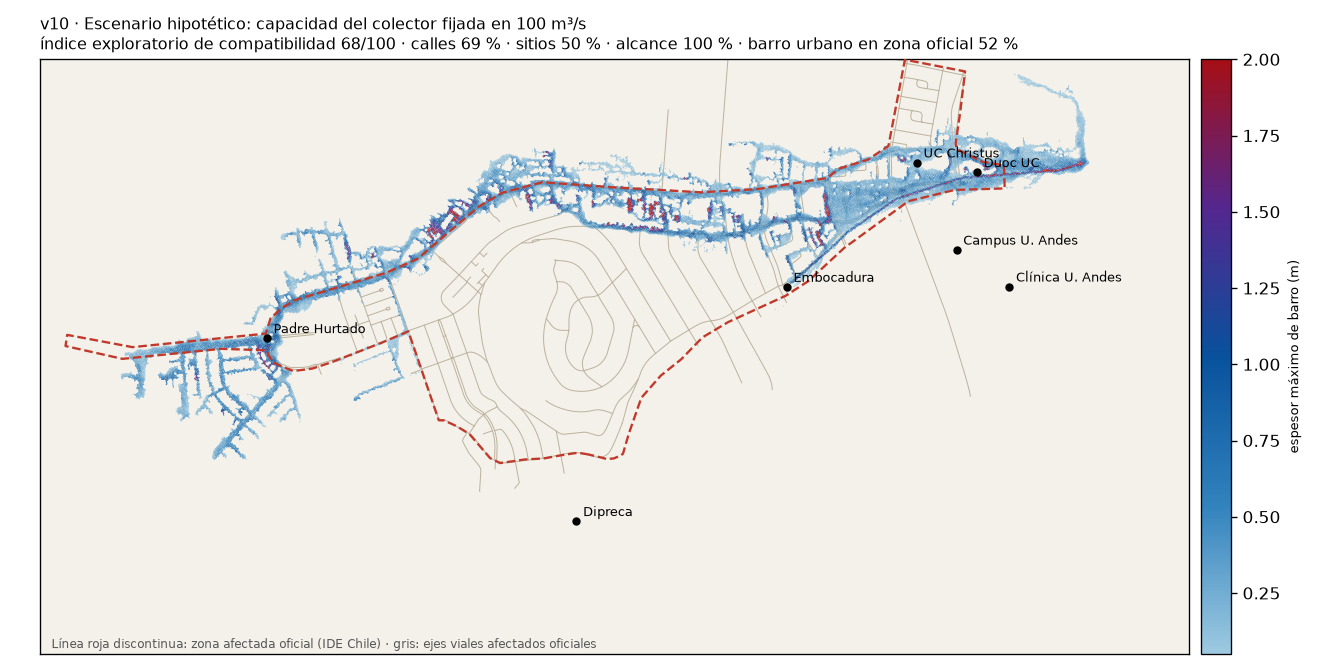
\includegraphics[width=\textwidth]{anexo/v10}\caption{Fact sheet v10: Hypothetical scenario: assumed culvert capacity set to 100 m$^3$/s.}\end{figure}

\subsection*{Mud type}

\paragraph{v08 · Thick mud (Glenwood 1, Cv 0.45).} \textbf{What it tests:} A more concentrated and viscous mud mixture (1,742 kg/m$^3$, yield stress 29 Pa). \textbf{What it shows:} Calculated: the front stops 396 m from Padre Hurtado. \textbf{Model limitations:} It does not meet the reach criterion. \textbf{What it raises:} An intermediate material (Cv 0.43, v25) does not reduce mud outside the official area; across the full Cv range from 0.24 to 0.48 (concentration quadrature), the index remains between 71 and 73. \textbf{Status:} Thicker variant: ECI 67/100.

\begin{figure}[H]\centering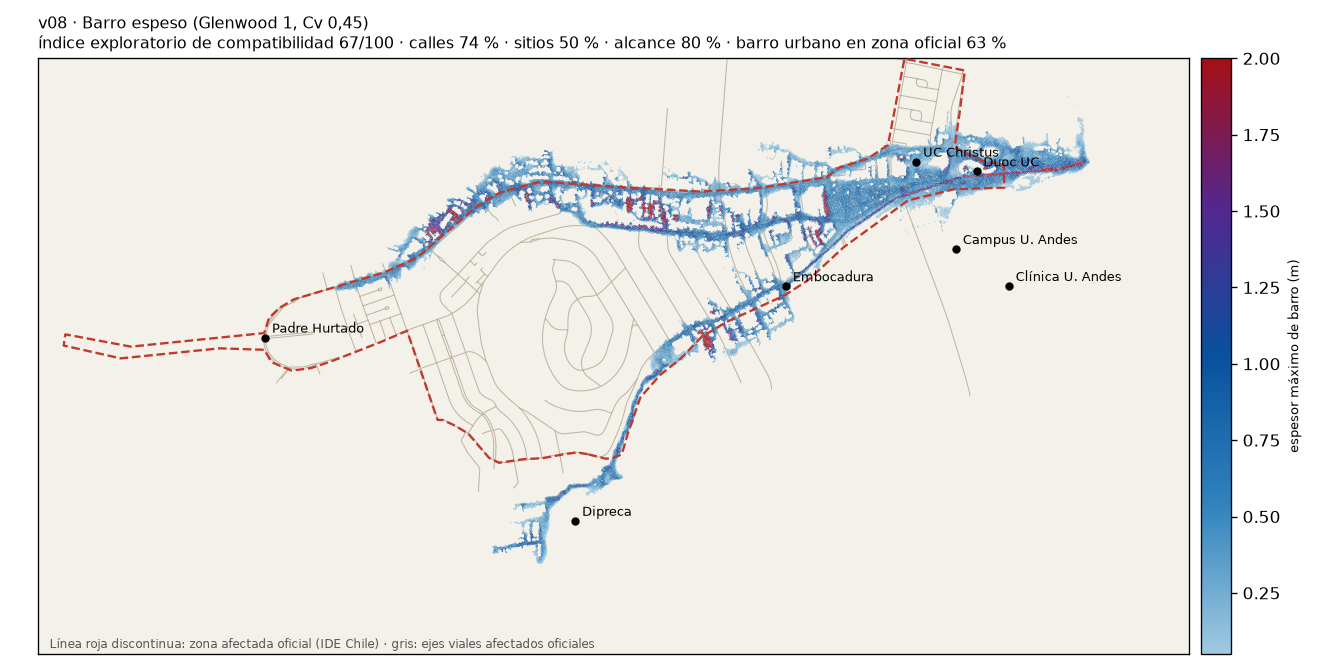
\includegraphics[width=\textwidth]{anexo/v08}\caption{Fact sheet v08: Thick mud (Glenwood 1, Cv 0.45).}\end{figure}

\paragraph{v09 · Very fluid mud (Aspen 2).} \textbf{What it tests:} A more fluid mud mixture than the reference. \textbf{What it shows:} Calculated: a result similar to the reference (ECI 70/100), with somewhat more mud inside the official area. \textbf{Model limitations:} It does not reach the southern sector (without southern branches or rainfall). \textbf{What it raises:} The ECI varies little between the materials tested; that variation alone does not summarize changes in reach, depth or velocity. \textbf{Status:} Index sensitivity to material: low. ECI 70/100.

\begin{figure}[H]\centering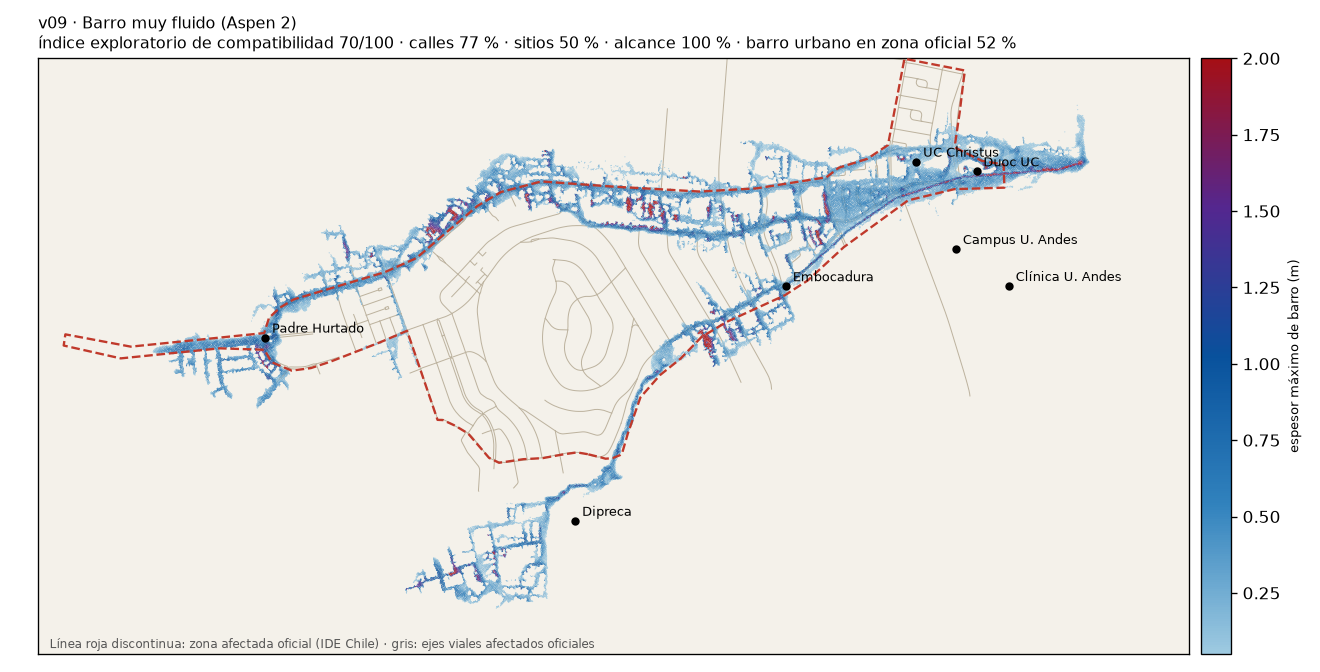
\includegraphics[width=\textwidth]{anexo/v09}\caption{Fact sheet v09: Very fluid mud (Aspen 2).}\end{figure}

\subsection*{Previous terrain (first model generation)}

\paragraph{e04 · Channel + culvert with assumed zero capacity, terrain with 1,103 buildings.} \textbf{What it tests:} The configuration selected in the first model generation (9 October), with only 1,103 buildings represented and the press-perimeter criterion. \textbf{What it shows:} Calculated: flow spreads more across the surface (93 ha inside the official area) in thinner layers and reaches Padre Hurtado. \textbf{Model limitations:} It calculates only 0.3 m around UC Christus (Cadena 3 reported about 1 m in the emergency department). \textbf{What it raises:} Representing all buildings changed the results; representation as impermeable blocks could intensify channeling compared with one that allows retention in buildings (v26). \textbf{Status:} Superseded by simulations with the full city: ECI 68/100.

\begin{figure}[H]\centering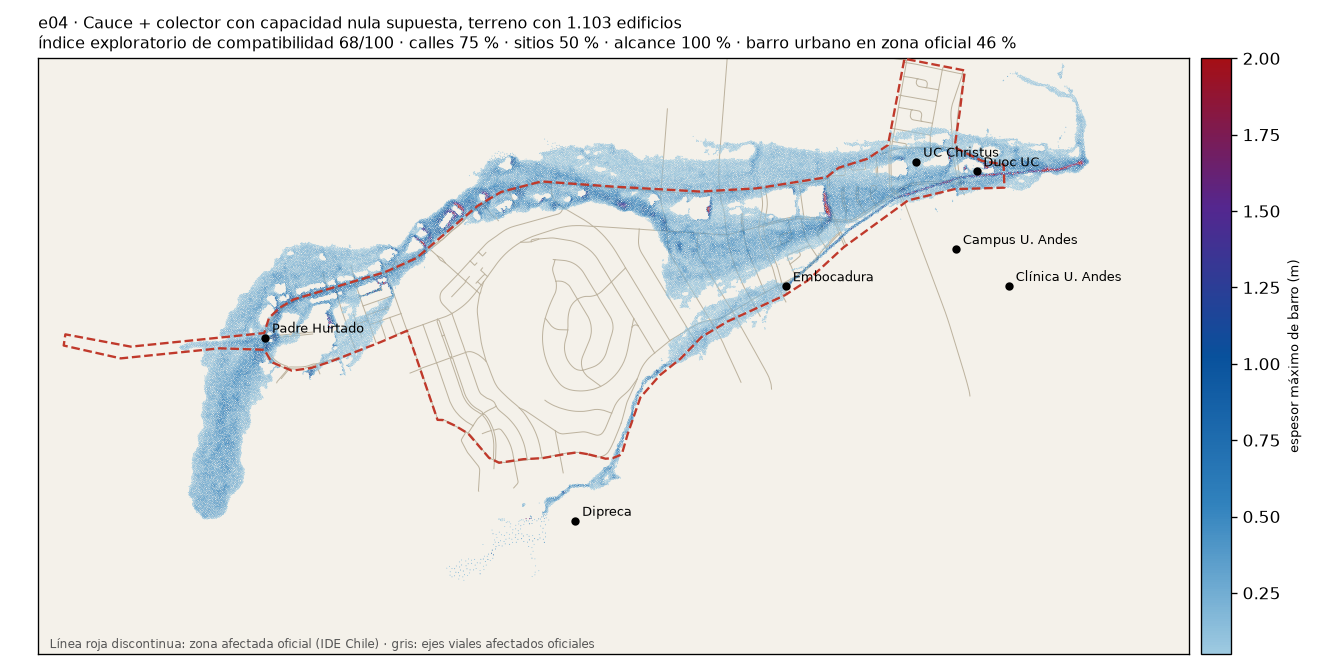
\includegraphics[width=\textwidth]{anexo/e04}\caption{Fact sheet e04: Channel + culvert with assumed zero capacity, terrain with 1,103 buildings.}\end{figure}

\paragraph{f03 · Alluvial fan + culvert inlet + hillside rainfall, previous terrain.} \textbf{What it tests:} The first simulation with hillside rainfall, using the previous terrain. \textbf{What it shows:} Calculated: it was the first to produce flow next to Clínica U. de los Andes and on La Plaza Sur. \textbf{Model limitations:} Low thickness around UC Christus and extent outside the official area. \textbf{What it raises:} It led to the hypothesis selected for the held-out test (channel + southern branches + rainfall, z02). \textbf{Status:} ECI 71/100.

\begin{figure}[H]\centering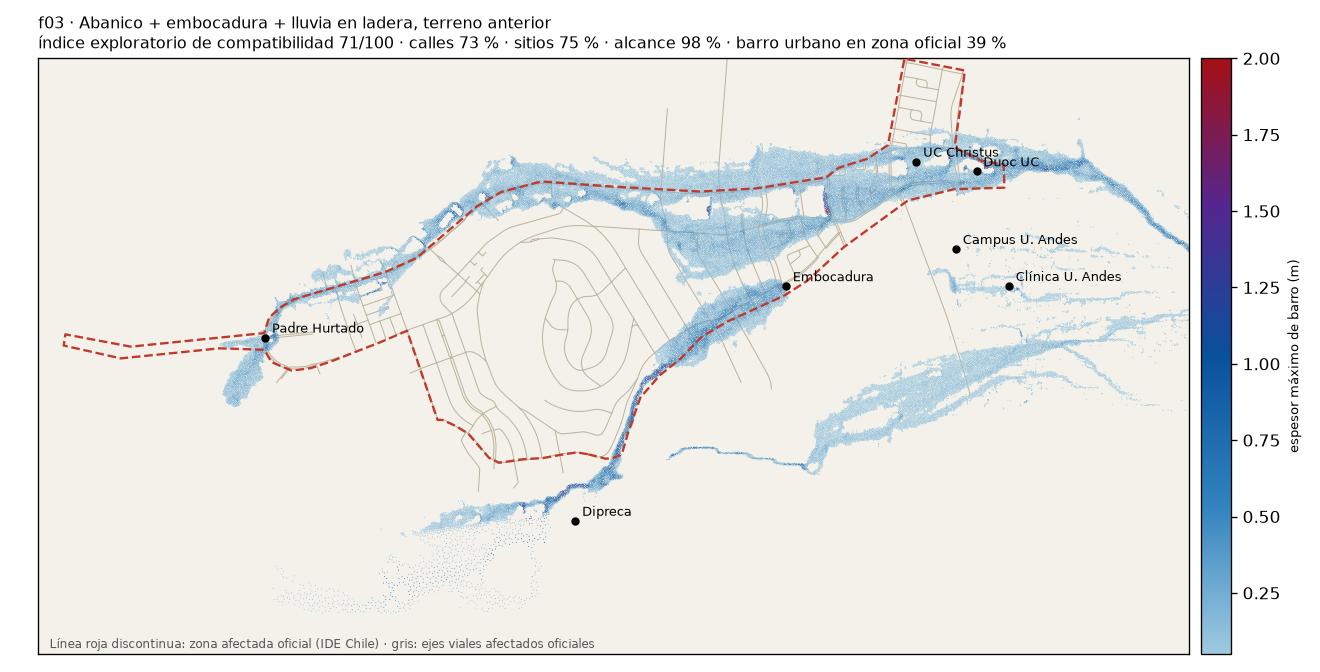
\includegraphics[width=\textwidth]{anexo/f03}\caption{Fact sheet f03: Alluvial fan + culvert inlet + hillside rainfall, previous terrain.}\end{figure}

\paragraph{e03 · Overflow at the culvert inlet only (H2).} \textbf{What it tests:} Surface inflow of the entire assumed volume at Francisco Bulnes Correa, without inferring the actual operation of the channel. \textbf{What it shows:} Calculated: it wets Quebrada Honda but none of the alluvial fan. \textbf{Model limitations:} It does not reproduce General Blanche, Camino El Alba, Duoc UC or UC Christus. \textbf{What it raises:} El Desconcierto reports an overflow at Bulnes Correa described by Carabineros. Simulation e03 alone does not reproduce the full set of observations. \textbf{Status:} Does not by itself reproduce the full set of observations under the assumptions and terrain of e03: ECI 16/100.

\begin{figure}[H]\centering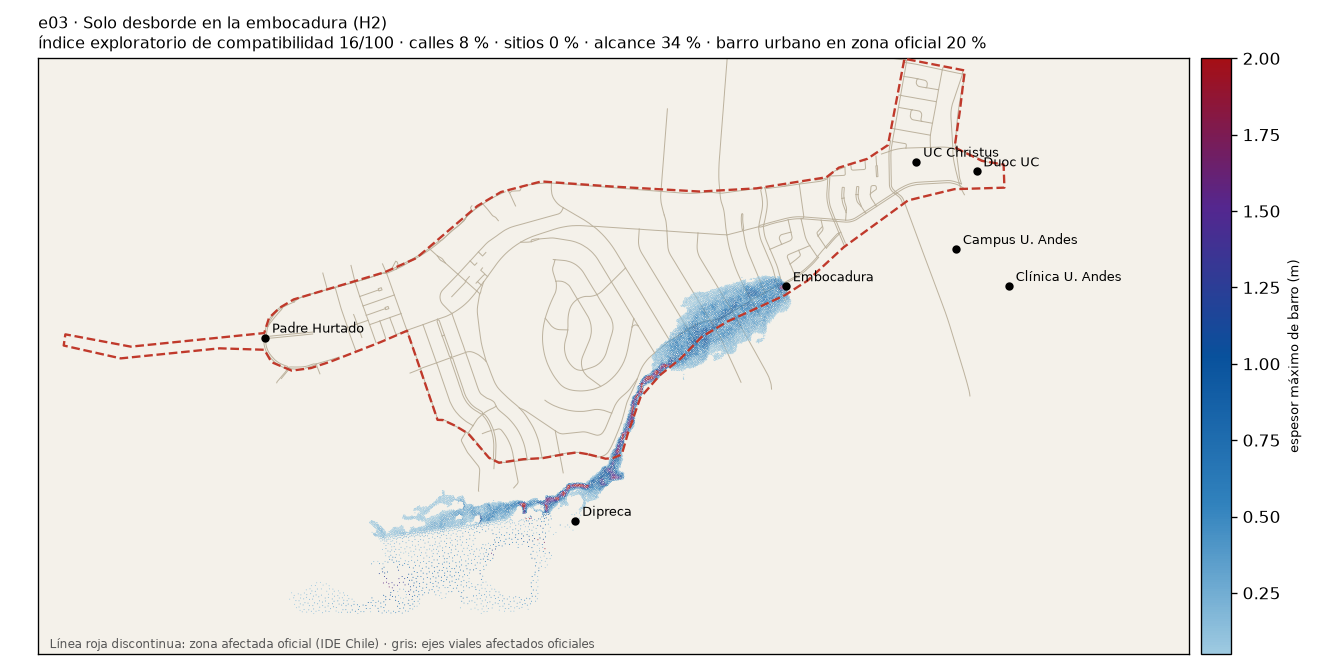
\includegraphics[width=\textwidth]{anexo/e03}\caption{Fact sheet e03: Overflow at the culvert inlet only (H2).}\end{figure}
